
%%--------------------------------------------------
%% CPO: Multiple Choice Questions
%%--------------------------------------------------


%% Chapter 3: Conservation Laws
%%--------------------------------------------------


%% Learning Objectives
%%--------------------------------------------------

%% Use Newton’s third law to explain various situations. 
%% Explain the relationship between the third law and conservation of momentum.
%% Solve momentum and impulse problems. 
%% Describe work and energy. 
%% Calculate potential and kinetic energy. 
%% Apply the law of conservation of energy to explain the motion of an object acted on by gravity. 
%% Distinguish between elastic and inelastic collisions.
%% Use momentum conservation to solve collision problems. 
%% Explain how momentum, impulse, force, and time are related.


%% CPO Multiple Choice Questions
%%--------------------------------------------------
\element{cpo-mc}{
\begin{question}{cpo-ch03-q01}
    As the speed of a rolling ball is increasing,
        the increasing speed is accompanied by:
    \begin{choices}
      \correctchoice{increasing momentum.}
        \wrongchoice{increasing inertia.}
        \wrongchoice{decreasing momentum.}
        \wrongchoice{both increasing inertia and momentum.}
    \end{choices}
\end{question}
}

\element{cpo-mc}{
\begin{question}{cpo-ch03-q02}
    ``Forces occur in pair'' is another way of stating Newton's:
    \begin{choices}
        \wrongchoice{First law of motion.}
        \wrongchoice{Second law of motion.}
      \correctchoice{Third law of motion.}
        \wrongchoice{Universal law of motion.}
    \end{choices}
\end{question}
}

\element{cpo-mc}{
\begin{question}{cpo-ch03-q03}
    Even though every action force has an equal but opposite reaction force,
        they do not cancel one another and motion may still occur because the:
    \begin{choices}
        \wrongchoice{Action and reaction forces are applied to the same object.}
      \correctchoice{Action and reaction forces are applied to different objects.}
        \wrongchoice{Two forces have different magnitudes.}
        \wrongchoice{Two forces have equal magnitudes.}
    \end{choices}
\end{question}
}

\element{cpo-mc}{
\begin{question}{cpo-ch03-q04}
    To calculate momentum:
    \begin{choices}
        \wrongchoice{Add the mass of an object to its inertia.}
        \wrongchoice{Add the mass of an object to its velocity.}
        \wrongchoice{Multiply the mass of an object by its inertia.}
      \correctchoice{Multiply the mass of an object by its velocity.}
    \end{choices}
\end{question}
}

\element{cpo-mc}{
\begin{question}{cpo-ch03-q05}
    The impulse applied to an object is equal to the change in the object's:
    \begin{multicols}{2}
    \begin{choices}
        \wrongchoice{mass.}
        \wrongchoice{inertia.}
      \correctchoice{momentum.}
        \wrongchoice{height.}
    \end{choices}
    \end{multicols}
\end{question}
}

\element{cpo-mc}{
\begin{questionmult}{cpo-ch03-Q06}
    To increase the final momentum of a racquetball,
        the player should:
    \begin{choices}
      \correctchoice{Swing the racquet as fast as possible.}
      \correctchoice{Follow through when hitting the ball.}
      \correctchoice{Increase contact time with the ball.}
    \end{choices}
\end{questionmult}
}

\element{cpo-mc}{
\begin{question}{cpo-ch03-q07}
    The impulse necessary to change the momentum of a \SI{20}{\kilo\gram} object by \SI{5}{\kilo\gram\meter\per\second} is:
    \begin{multicols}{2}
    \begin{choices}
        \wrongchoice{\SI{4}{\kilo\gram\meter\per\second}.}
      \correctchoice{\SI{5}{\kilo\gram\meter\per\second}.}
        \wrongchoice{\SI{15}{\kilo\gram\meter\per\second}.}
        \wrongchoice{\SI{100}{\kilo\gram\meter\per\second}.}
    \end{choices}
    \end{multicols}
\end{question}
}

\element{cpo-mc}{
\begin{question}{cpo-ch03-q08}
    A rocket can fly into space because:
    \begin{choices}
        \wrongchoice{The exhaust gases push against the ground and the ground, in turn, pushed the rocket.}
      \correctchoice{The rocket pushed on exhaust gases and the exhaust gases push back on the rocket.}
        \wrongchoice{As the fuel burns, the rocket's mass decreases reducing the force of gravity on the rocket.}
        \wrongchoice{The launch pad absorbs momentum that it imparts to the rocket.}
    \end{choices}
\end{question}
}

\element{cpo-mc}{
\begin{question}{cpo-ch03-q09}
    The momentum of a \SI{2000}{\kilo\gram} car traveling at \SI{20}{\meter\per\second} is:
    \begin{multicols}{2}
    \begin{choices}
        \wrongchoice{\SI{0}{\kilo\gram\meter\per\second}.}
        \wrongchoice{\SI{0.001}{\kilo\gram\meter\per\second}.}
        \wrongchoice{\SI{100}{\kilo\gram\meter\per\second}.}
      \correctchoice{\SI{40 000}{\kilo\gram\meter\per\second}.}
    \end{choices}
    \end{multicols}
\end{question}
}

\element{cpo-mc}{
\begin{question}{cpo-ch03-q10}
    If a \SI{40 000}{\kilo\gram} rocket were traveling from its launch pad at a speed of \SI{150}{\meter\per\second},
        \SI{800}{\kilo\gram} of gases would be expelled from the rocket at a speed of about:
    \begin{multicols}{2}
    \begin{choices}
        \wrongchoice{\SI{0.33}{\meter\per\second}.}
        \wrongchoice{\SI{270}{\meter\per\second}.}
      \correctchoice{\SI{7 500}{\meter\per\second}.}
        \wrongchoice{\SI{21 000}{\meter\per\second}.}
    \end{choices}
    \end{multicols}
\end{question}
}

\element{cpo-mc}{
\begin{question}{cpo-ch03-q11}
    Air bags reduce injury in automobile accidents by:
    \begin{choices}
        \wrongchoice{Reducing the time of collision.}
        \wrongchoice{Reducing the change in momentum.}
        \wrongchoice{Increasing the applied force.}
      \correctchoice{Increasing the time of collision.}
    \end{choices}
\end{question}
}

\element{cpo-mc}{
\begin{question}{cpo-ch03-q12}
    Ken rolls a \SI{7}{\kilo\gram} bowling ball so slowly that it stops before it moves through all of the pins.
    The impulse necessary to stop this bowling ball rolling at \SI{2}{\meter\per\second} is:
    \begin{multicols}{2}
    \begin{choices}
      \correctchoice{\SI{3.5}{\newton\second}.}
        \wrongchoice{\SI{5.0}{\newton\second}.}
        \wrongchoice{\SI{7.0}{\newton\second}.}
        \wrongchoice{\SI{14}{\newton\second}.}
    \end{choices}
    \end{multicols}
\end{question}
}

\element{cpo-mc}{
\begin{question}{cpo-ch03-q13}
    Kiki accidentally nudges a glass tumbler with her elbow and it falls toward a hard, ceramic tile floor.
    As a soccer player, Kiki reacts by catching the glass with her foot and lowering it to the floor,
        preventing the glass from breaking.
    Her action prevents the breakage because:
    \begin{choices}
        \wrongchoice{The change in momentum is smaller when Kiki catches and lowers the glass to the floor.}
        \wrongchoice{The impulse is smaller when Kiki catches the glass and lowers is to the floor.}
      \correctchoice{The time interval for stopping is greater when Kiki catches the glass with her foot.}
        \wrongchoice{A larger force is exerted by Kiki's foot to stop the glass in time.}
    \end{choices}
\end{question}
}

\element{cpo-mc}{
\begin{question}{cpo-ch03-q14}
    While standing on a stationary skateboard, Jolene tosses a heavy ball horizontally toward one end of her skateboard.
    The skateboard moves.
    Assuming there is no friction in the system when the ball is tossed, which statement about the momentum of the heavy ball is \emph{incorrect}?
    \begin{choices}
        \wrongchoice{The ball's momentum is equal in size to the momentum of Jolene and her skateboard.}
        \wrongchoice{The ball's momentum plus the momentum of Jolene and her skateboard equals zero.}
        \wrongchoice{The ball's momentum has increased because Jolene has tossed it.}
      \correctchoice{The direction of the ball's momentum and Jolene's momentum are the same.}
    \end{choices}
\end{question}
}

\element{cpo-mc}{
\begin{question}{cpo-ch03-q15}
    Alex hits a line drive directly up the middle which leaves his bat traveling at \SI{250}{\meter\per\second}.
    If the pitcher has thrown the \SI{0.15}{\kilo\gram} baseball to Alex at \SI{140}{\meter\per\second},
        what is the impulse applied to the baseball by Alex?
    \begin{multicols}{2}
    \begin{choices}
      \correctchoice{\SI{17}{\newton\second}}
        \wrongchoice{\SI{21}{\newton\second}}
        \wrongchoice{\SI{38}{\newton\second}}
        \wrongchoice{\SI{59}{\newton\second}}
    \end{choices}
    \end{multicols}
\end{question}
}

\element{cpo-mc}{
\begin{question}{cpo-ch03-q16}
    A \SI{0.15}{\kilo\gram} baseball thrown at a speed of \SI{50}{\meter\per\second} and a \SI{7.15}{\kilo\gram} bowling ball rolling at \SI{2}{\meter\per\second} are both stopped in \SI{0.2}{\second}.
    \begin{choices}
        \wrongchoice{The baseball is stopped with less force because it has less inertia.}
      \correctchoice{The baseball is stopped with less force because it has less momentum.}
        \wrongchoice{The bowling ball is stopped with less force because it has less momentum.}
        \wrongchoice{The bowling ball is stopped with less force because it has less inertia.}
    \end{choices}
\end{question}
}

\element{cpo-mc}{
\begin{question}{cpo-ch03-q17}
    What impulse must be applied to a \SI{3.0}{\kilo\gram} object to give it \SI{150}{\joule} of kinetic energy?
    \begin{multicols}{2}
    \begin{choices}
        \wrongchoice{\SI{21}{\newton\second}}
      \correctchoice{\SI{30}{\newton\second}}
        \wrongchoice{\SI{50}{\newton\second}}
        \wrongchoice{\SI{3 000}{\newton\second}}
    \end{choices}
    \end{multicols}
\end{question}
}

\element{cpo-mc}{
\begin{question}{cpo-ch03-q18}
    The skateboard on which you are standing moves as one of your feet pushes on the ground because the force you apply on the skateboard:
    \begin{choices}
        \wrongchoice{Equals the force applied to you by the skateboard.}
        \wrongchoice{Is larger than the force applied to you by the skateboard.}
      \correctchoice{Equals the force applied by the ground on the skateboard.}
        \wrongchoice{Is larger than the force applied by the ground on the skateboard.}
    \end{choices}
\end{question}
}

\element{cpo-mc}{
\begin{question}{cpo-ch03-q19}
    Jumping on a trampoline, Jeffrey can easily soar \SI{5}{\foot} into the air but can only jump \SI{2}{\foot} from the blacktop of the driveway basketball court because the:
    \begin{choices}
        \wrongchoice{Court applied a larger impulse.}
      \correctchoice{Trampoline applies a larger impulse.}
        \wrongchoice{Court applies less force on Jeffrey.}
        \wrongchoice{Trampoline applies more force on Jeffrey.}
    \end{choices}
\end{question}
}

\element{cpo-mc}{
\begin{question}{cpo-ch03-q20}
    Energy that is stored due to the position of an object may be called \rule[-0.1pt]{4em}{0.1pt} energy.
    \begin{multicols}{2}
    \begin{choices}
        \wrongchoice{kinetic}
      \correctchoice{potential}
        \wrongchoice{radiant}
        \wrongchoice{nuclear}
    \end{choices}
    \end{multicols}
\end{question}
}

\element{cpo-mc}{
\begin{question}{cpo-ch03-q21}
    A \SI{20}{\kilo\gram} object falls \SI{2.0}{\meter} to the floor.
    At what point in its fall does the kinetic energy of a body equal its potential energy?
    \begin{choices}
        \wrongchoice{At all points of its fall.}
        \wrongchoice{Very nearly at the top of the fall.}
      \correctchoice{Halfway to the floor.}
        \wrongchoice{Just the instant before it hits the floor.}
    \end{choices}
\end{question}
}

\element{cpo-mc}{
\begin{question}{cpo-ch03-q22}
    An object falls without friction near the Earth's surface.
    The loss of its potential energy is equal to its:
    \begin{choices}
        \wrongchoice{loss of height.}
        \wrongchoice{loss of mass.}
      \correctchoice{gain in kinetic energy.}
        \wrongchoice{gain in velocity.}
    \end{choices}
\end{question}
}

\element{cpo-mc}{
\begin{question}{cpo-ch03-q23}
    The diagram below represents a cart traveling from left to right along a frictionless surface with an initial speed of \SI{3}{\meter\per\second}.
    \begin{center}
    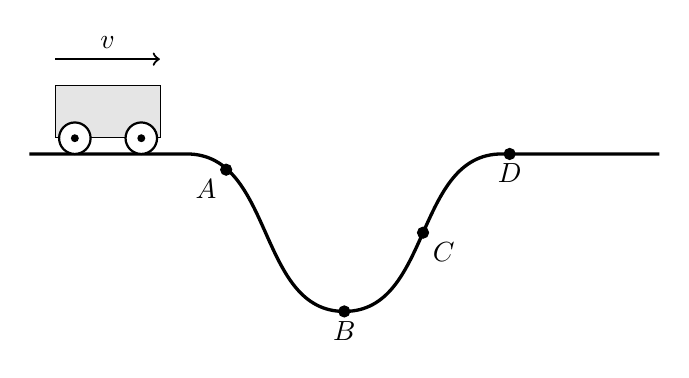
\begin{tikzpicture}
        %% Path
        \draw[very thick] (-4,0) -- (-2,0) to[out=0,in=180] (0,-2) to[out=0,in=180] (2,0) to (4,0);
        %% Cart
        \node[draw,fill=white!90!black,minimum width=1.33cm,minimum height=0.66cm,anchor=south] (A) at (-3,0.2) {};
        %% wheels
        \draw[thick,fill=white] (A.south east) ++(180:0.25) circle (0.2cm);
        \draw[thick,fill] (A.south east) ++(180:0.25) circle (1pt);
        \draw[thick,fill=white] (A.south west) ++(0:0.25) circle (0.2cm);
        \draw[thick,fill] (A.south west) ++(0:0.25) circle (1pt);
        %% Velocity
        \draw[thick,->] (A.north west) ++(90:0.33) --++(0:1.33) node[pos=0.5,anchor=south] {$v$};
        %% Labels
        \draw[fill] (-1.5,-0.2) circle (2pt) node[anchor=north east] {$A$};
        \draw[fill] (0,-2) circle (2pt) node[anchor=north] {$B$};
        \draw[fill] (1,-1) circle (2pt) node[anchor=north west] {$C$};
        \draw[fill] (2.1,0) circle (2pt) node[anchor=north] {$D$};
    \end{tikzpicture}
    \end{center}
    At what point is the potential energy least?
    \begin{multicols}{4}
    \begin{choices}[o]
        \wrongchoice{$A$}
      \correctchoice{$B$}
        \wrongchoice{$C$}
        \wrongchoice{$D$}
    \end{choices}
    \end{multicols}
\end{question}
}

\element{cpo-mc}{
\begin{question}{cpo-ch03-q24}
    The ability to cause change is defined as:
    \begin{choices}
        \wrongchoice{force and is measured in newtons.}
        \wrongchoice{power and is measured in watts.}
      \correctchoice{energy and is measured in joules.}
        \wrongchoice{impulse and is measured in newton-seconds.}
    \end{choices}
\end{question}
}

\element{cpo-mc}{
\begin{question}{cpo-ch03-q25}
    Work may be measured using units of:
    \begin{choices}
        \wrongchoice{watt (\si{\watt})}
        \wrongchoice{newton (\si{\newton})}
      \correctchoice{joule (\si{\joule})}
        \wrongchoice{newton per second (\si{\newton\per\second})}
    \end{choices}
\end{question}
}

\element{cpo-mc}{
\begin{question}{cpo-ch03-q26}
    In science, work is defined as:
    \begin{choices}
        \wrongchoice{The mass of an object multiplied by its acceleration.}
        \wrongchoice{The mass of an object multiplied by the force required to move it.}
        \wrongchoice{Force multiplied by the distance moved in a direction perpendicular to the force.}
      \correctchoice{Force multiplied by the distance moved in the same direction as the force.}
    \end{choices}
\end{question}
}

\element{cpo-mc}{
\begin{question}{cpo-ch03-q27}
    Potential energy increases as a marble:
    \begin{choices}
      \correctchoice{Slows rolling up an incline.}
        \wrongchoice{Increases speed down an incline.}
        \wrongchoice{Rolls at uniform speed on a level table.}
        \wrongchoice{Sits motionless on the floor.}
    \end{choices}
\end{question}
}

\element{cpo-mc}{
\begin{question}{cpo-ch03-q28}
    Calculate the work done to lift a barbell weighing \SI{100}{\newton} a distance of \SI{1.5}{\meter}.
    \begin{multicols}{2}
    \begin{choices}
        \wrongchoice{\SI{0.015}{\joule}}
      \correctchoice{\SI{15}{\joule}}
        \wrongchoice{\SI{66.7}{\joule}}
        \wrongchoice{\SI{150}{\joule}}
    \end{choices}
    \end{multicols}
\end{question}
}

\element{cpo-mc}{
\begin{question}{cpo-ch03-q29}
    John is pushing his younger sister, Jessica, on a swing.
    If Jessica weighs \SI{350}{\newton},
        how much higher above the ground must Jonah push her to increase her potential energy by \SI{525}{\joule}?
    \begin{multicols}{2}
    \begin{choices}
        \wrongchoice{\SI{0.67}{\meter}}
      \correctchoice{\SI{1.5}{\meter}}
        \wrongchoice{\SI{3.6}{\meter}}
        \wrongchoice{\SI{5.4}{\meter}}
    \end{choices}
    \end{multicols}
\end{question}
}

\element{cpo-mc}{
\begin{question}{cpo-ch03-q30}
    A basketball player who weighs \SI{600}{\newton} jumps \SI{0.5}{\meter} vertically off the floor.
    What is her kinetic energy the instant before hitting the floor?
    \begin{multicols}{2}
    \begin{choices}
        \wrongchoice{\SI{30}{\joule}}
        \wrongchoice{\SI{60}{\joule}}
      \correctchoice{\SI{300}{\joule}}
        \wrongchoice{\SI{600}{\joule}}
    \end{choices}
    \end{multicols}
\end{question}
}

\element{cpo-mc}{
\begin{question}{cpo-ch03-q31}
    Lifting a \SI{70}{\kilo\gram} barbell \SI{2.0}{\meter} above the floor increases its potential energy by about:
    \begin{multicols}{2}
    \begin{choices}
        \wrongchoice{\SI{35}{\joule}}
        \wrongchoice{\SI{140}{\joule}}
        \wrongchoice{\SI{350}{\joule}}
      \correctchoice{\SI{1 400}{\joule}}
    \end{choices}
    \end{multicols}
\end{question}
}

\element{cpo-mc}{
\begin{question}{cpo-ch03-q32}
    The amount of mechanical kinetic energy possessed by a \SI{0.25}{\kilo\gram} ball rolling at a speed of \SI{2.5}{\meter\per\second} is:
    \begin{multicols}{2}
    \begin{choices}
        \wrongchoice{\SI{0.31}{\joule}}
        \wrongchoice{\SI{0.63}{\joule}}
      \correctchoice{\SI{0.78}{\joule}}
        \wrongchoice{\SI{1.6}{\joule}}
    \end{choices}
    \end{multicols}
\end{question}
}

\element{cpo-mc}{
\begin{question}{cpo-ch03-q33}
    As the speed of a moving object doubles,
        the amount of mechanical kinetic energy that is possesses:
    \begin{choices}
        \wrongchoice{increases by two times.}
      \correctchoice{increases by four times.}
        \wrongchoice{decreases by two times.}
        \wrongchoice{decreases by four times.}
    \end{choices}
\end{question}
}

\element{cpo-mc}{
\begin{question}{cpo-ch03-q34}
    Jonah is pushing his younger sister, Jessica, on a swing.
    If Jessica has a mass of \SI{35}{\kilo\gram},
        how much higher above ground must Jonah pusher her to increase her potential energy by \SI{525}{\joule}?
    \begin{multicols}{2}
    \begin{choices}
        \wrongchoice{\SI{0.67}{\meter}.}
      \correctchoice{\SI{1.5}{\meter}.}
        \wrongchoice{\SI{3.6}{\meter}.}
        \wrongchoice{\SI{5.4}{\meter}.}
    \end{choices}
    \end{multicols}
\end{question}
}

\element{cpo-mc}{
\begin{question}{cpo-ch03-q35}
    Shawna, who weighs \SI{54}{\kilo\gram}, is roller blading on a level surface.
    If she is rolling at \SI{12}{\meter\per\second},
        to what height would she roll up an incline before stopping?
    (Assume there is no friction)
    \begin{multicols}{2}
    \begin{choices}
        \wrongchoice{\SI{0.61}{\meter}.}
        \wrongchoice{\SI{1.2}{\meter}.}
      \correctchoice{\SI{7.3}{\meter}.}
        \wrongchoice{\SI{15}{\meter}.}
    \end{choices}
    \end{multicols}
\end{question}
}

\element{cpo-mc}{
\begin{question}{cpo-ch03-q36}
    When the brakes are fully applied, compared to the distance required to stop a car going \SI{30}{mile\per\hour},
        the distance needed to stop a car going \SI{90}{mile\per\hour} is:
    \begin{multicols}{2}
    \begin{choices}
        \wrongchoice{3 times as great}
        \wrongchoice{6 times as great}
      \correctchoice{9 times as great}
        \wrongchoice{the same}
    \end{choices}
    \end{multicols}
\end{question}
}

\element{cpo-mc}{
\begin{question}{cpo-ch03-q37}
    All of the following may be the result of an inelastic collision \emph{except}:
    \begin{choices}
        \wrongchoice{permanent change in the shape of the colliding bodies.}
        \wrongchoice{kinetic energy released as sound.}
        \wrongchoice{colliding bodies stick to one another.}
      \correctchoice{zero loss of kinetic energy.}
    \end{choices}
\end{question}
}

\element{cpo-mc}{
\begin{question}{cpo-ch03-q38}
    Which of the following situations is an example of a mostly elastic collision?
    \begin{choices}
      \correctchoice{Two billiard balls collide and bounce off each other.}
        \wrongchoice{Two train card collide and stick together.}
        \wrongchoice{When a soft piece of clay falls onto the floor, its shape flattens.}
        \wrongchoice{A glass falls off the table and breaks.}
    \end{choices}
\end{question}
}

\element{cpo-mc}{
\begin{question}{cpo-ch03-q39}
    When two objects hit each other, a(n) \rule[-0.1pt]{4em}{0.1pt} occurs.
    \begin{multicols}{2}
    \begin{choices}
        \wrongchoice{joule}
        \wrongchoice{impulse}
      \correctchoice{collision}
        \wrongchoice{momentum}
    \end{choices}
    \end{multicols}
\end{question}
}

\element{cpo-mc}{
\begin{question}{cpo-ch03-q40}
    A boy whose mass is \SI{40}{\kilo\gram} runs at \SI{5}{\meter\per\second} and jumps onto a \SI{10}{\kilo\gram} stationary sled.
    The boy slides on the sled over a horizontal, frictionless surface at a speed of:
    \begin{multicols}{2}
    \begin{choices}
        \wrongchoice{\SI{2}{\meter\per\second}.}
      \correctchoice{\SI{4}{\meter\per\second}.}
        \wrongchoice{\SI{5}{\meter\per\second}.}
        \wrongchoice{\SI{10}{\meter\per\second}.}
    \end{choices}
    \end{multicols}
\end{question}
}

\element{cpo-mc}{
\begin{question}{cpo-ch03-q41}
    What braking force is needed to stop a \SI{1 000}{\kilo\gram} car moving at \SI{10}{\meter\per\second} in a time of \SI{1}{\second}?
    \begin{multicols}{2}
    \begin{choices}
        \wrongchoice{\SI{1}{\newton}}
        \wrongchoice{\SI{10}{\newton}}
        \wrongchoice{\SI{100}{\newton}}
      \correctchoice{\SI{10 000}{\newton}}
    \end{choices}
    \end{multicols}
\end{question}
}

\element{cpo-mc}{
\begin{question}{cpo-ch03-q42}
    A \SI{2}{\kilo\gram} piece of clay moving at \SI{4}{\meter\per\second} strikes and sticks to a second \SI{4}{\kilo\gram} piece of clay moving at \SI{1}{\meter\per\second} in the opposite direction.
    Calculate the speed of the combined piece of clay.
    \begin{multicols}{2}
    \begin{choices}
        \wrongchoice{\SI{1}{\meter\per\second}}
      \correctchoice{\SI{2}{\meter\per\second}}
        \wrongchoice{\SI{4}{\meter\per\second}}
        \wrongchoice{\SI{6}{\meter\per\second}}
    \end{choices}
    \end{multicols}
\end{question}
}

\endinput

